
\documentclass[dvipdfmx]{standalone}
\usepackage[T1]{fontenc}
\usepackage{newtxtext, newtxmath}

\usepackage{tikz}
\usetikzlibrary{shapes.multipart}
\usetikzlibrary{arrows}

\newcommand{\ClassDiagram}[5]{%
  node (#1) [rectangle split, rectangle split parts=3, draw, align=center, text width=#2]
  { #3
    \nodepart[align=left]{two}
    #4
    \nodepart[align=left]{three}
    #5
  };
}

\begin{document}
  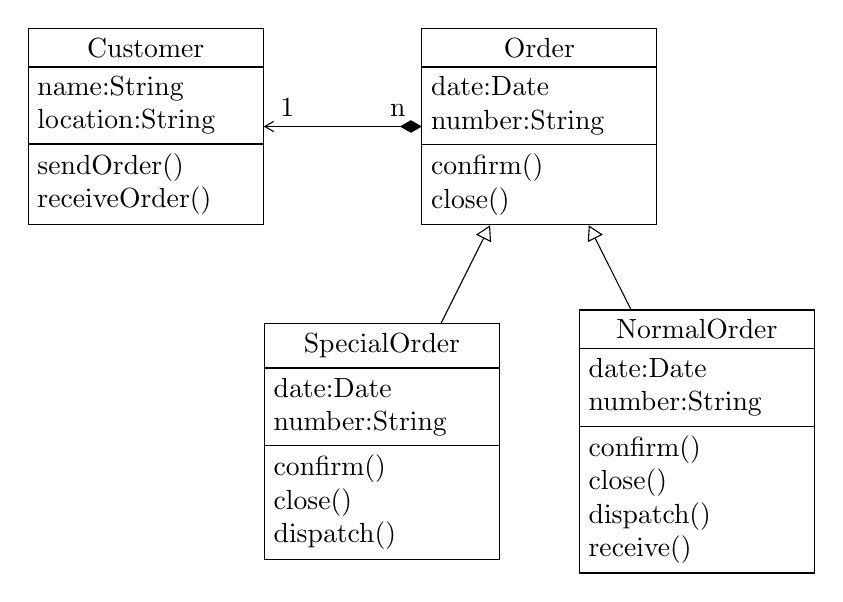
\begin{tikzpicture}
    \draw (5,5) \ClassDiagram{order}{2.75cm}
      {Order}{date:Date\\number:String}{confirm()\\close()}
    \draw (3,1) \ClassDiagram{special order}{2.75cm}
      {SpecialOrder}{date:Date\\number:String}{confirm()\\close()\\dispatch()}
    \draw (7,1) \ClassDiagram{normal order}{2.75cm}
      {NormalOrder}{date:Date\\number:String}{confirm()\\close()\\dispatch()\\receive()}

    \draw (0,5) \ClassDiagram{customer}{2.75cm}
      {Customer}{name:String\\location:String}{sendOrder()\\receiveOrder()}

    \draw[->, > = open triangle 60] (special order) -- (order);
    \draw[->, > = open triangle 60] (normal order) -- (order);
    \draw[<->, arrows = diamond - angle 60]
      (order) -- (customer) node[above, pos=0.15]{n} node[above, pos=0.85]{1};
  \end{tikzpicture}
\end{document}
